% !Mode:: "TeX:UTF-8"

\chapter{分层的动态温度管理方法}\label{sec:new_method}

在这一章,针对高性能众核微处理器,提出了新的分层动态温度管理方法。新方法是基于模型预测控制而且采用了任务迁移和DVFS。

众核处理器上执行结合任务迁移的MPC是一个挑战,因为但处理器处理器核数非常的大,
用复杂度为$O(n^{3})$的匈牙利算法计算任务迁移的决策需要花费大量的时间,这个时间可以看成是二部图匹配的时间。
为了扩展到具有大量处理器核的众核处理器,新的方法将处理器分成块,在两个层次上进行任务迁移决策:块内(低层)和块间(高层)。
首先在低层,也就是块内执行当前功耗和期望功耗组成的二部图匹配。在低层内没有匹配上的功耗元素,收集起来形成高层,也就是块间。
在高层,用改进的迭代最小割算法将高层分成“优化”块,在每个“优化”块执行二部图匹配。
高层最后没有匹配的功耗元素用DVFS来处理,以保证绝对的温度安全。
分层算法通过减小二部图匹配规模来降低计算开销,而且匹配是并行执行的,大大减少了计算时间,所以该算法可以扩展到众核系统。

\section{低层块内任务迁移}\label{sec:parts}

首先,我们将众核处理器分割成块。作为第一步,我们可以简单根据核的位置分割处理器。
就是在空间上直接划分处理器成块。
这一步分割不需要任何开销。我们通常将方形的块叫普通块,在边缘可能会出现矩形或者小的方形块,把这些称作边缘块。

块内匹配就是执行\ref{sec:dtm_mpc} 节中说明了二部图匹配的过程,这个叫做低层匹配。对每一个块,指定一个块内的核执行匹配的计算。
从整个芯片来看,低层匹配的计算是并行执行的。所以底层匹配引入的延迟时间只是一个普通块低层匹配的时间(注意,边缘块比常规快要小,也就是说它们的计算时间也并不计算在内)。

可以调整块内的核数以实现整个算法更小的延迟时间:如果核数很大,低层的功耗匹配将会占用更多的时间,
但是可以发现更多的匹配对,将会剩余更少的未匹配功耗到高层,这样高层匹配处理时间就会减少。

图~\ref{fig:cpu_partition} (a)是一个简单的低层划分的例子。这是一个100核微处理器,被划分为四个16核普通块(标记为A、B、D、E),五个核数4到8核的边缘块(标记为C、F、G、H、I)。
低层的功耗匹配将在每一个块内执行。图~\ref{fig:bi2} 展示的正是图~\ref{fig:cpu_partition} (a)中块I内的二部图匹配。

\begin{figure}[H]
  \centering
    \subfigure[微处理器分割成块准备进行低层二部图匹配。]
  {
    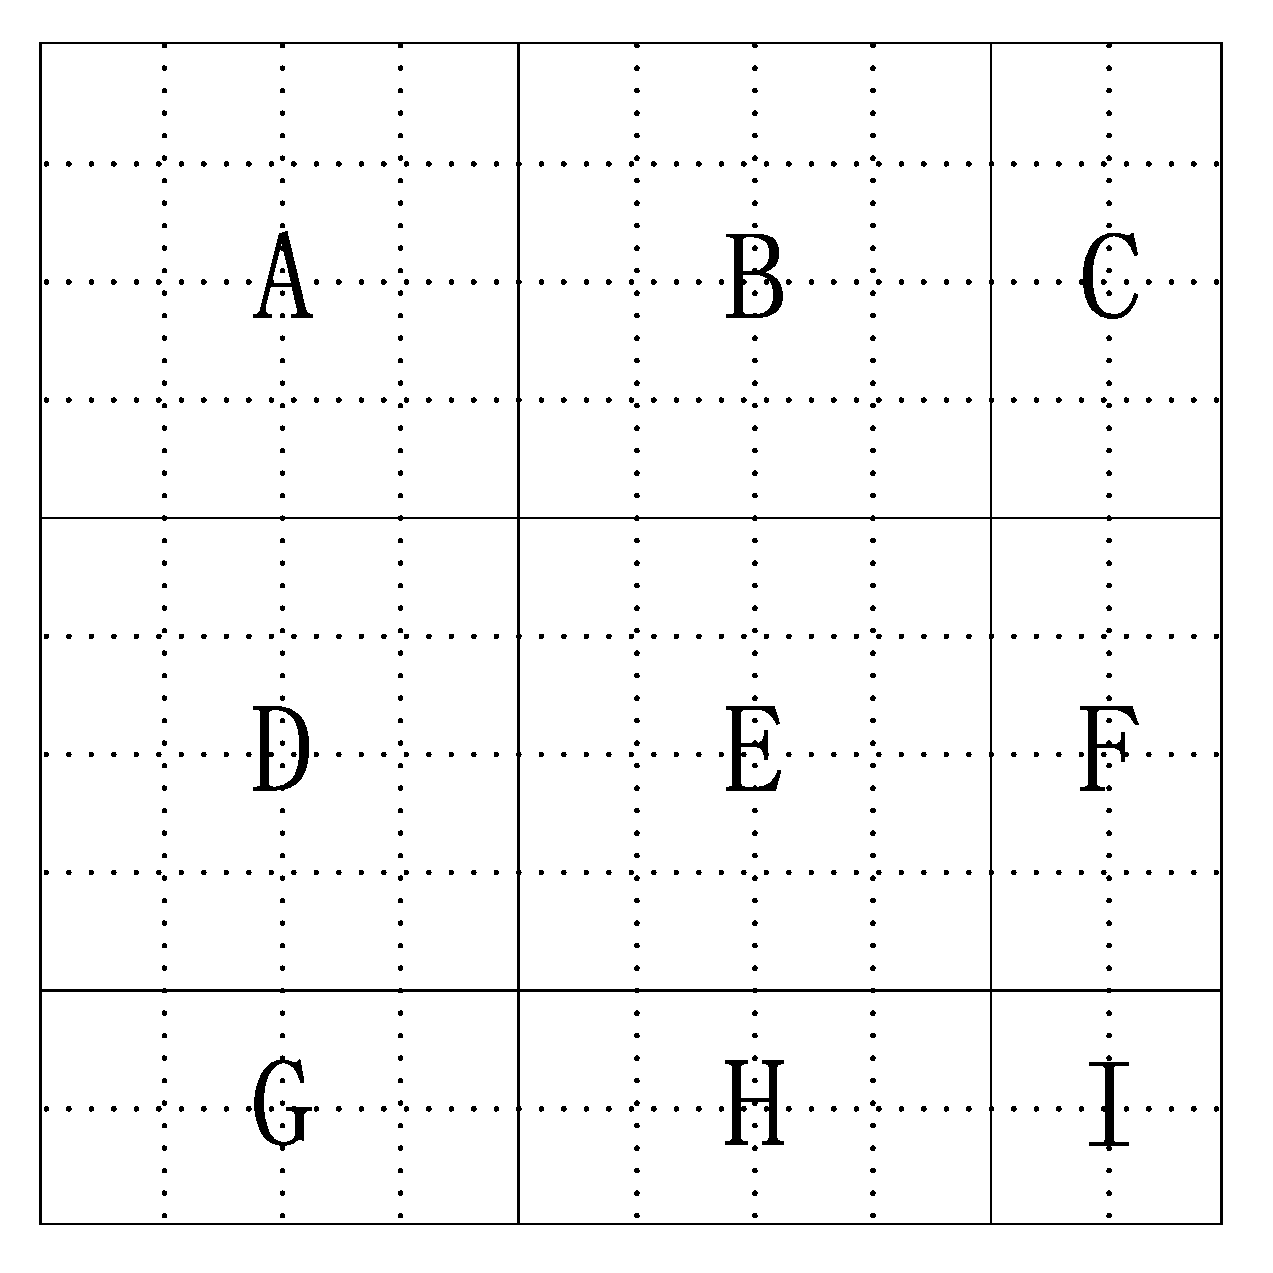
\includegraphics[width=0.32\columnwidth]{fig/part1}
  }
  \subfigure[低层二部图匹配之后留下的未匹配核(红色)。]
  {
    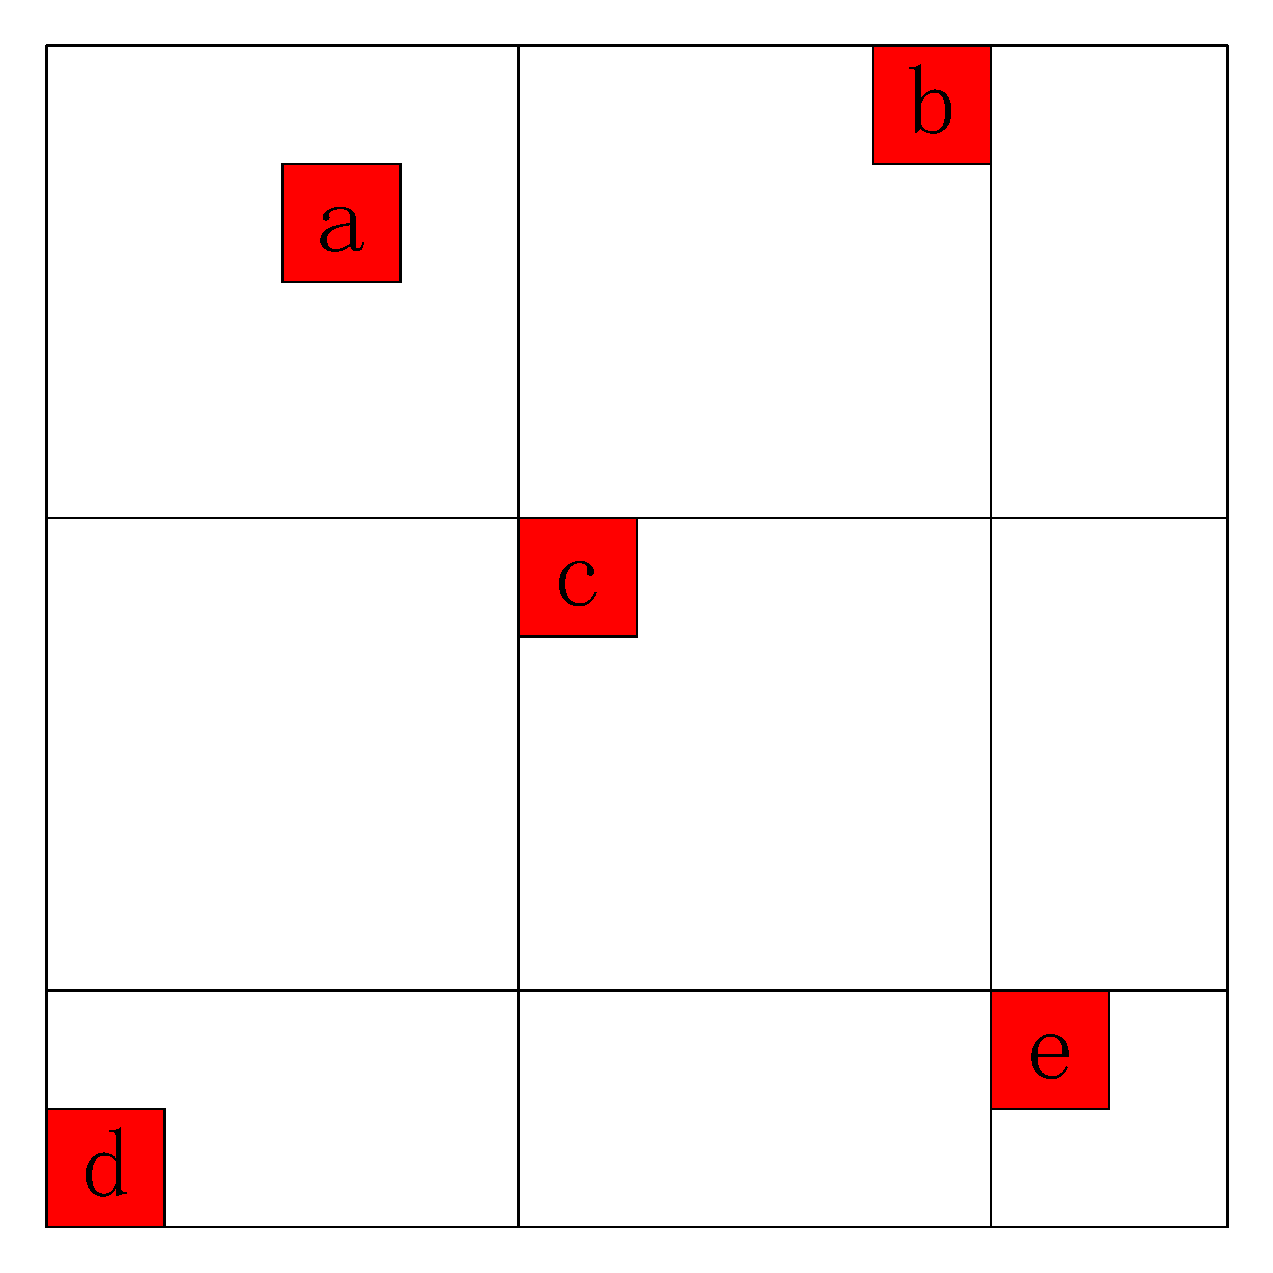
\includegraphics[width=0.32\columnwidth]{fig/partmod}
  }
  \caption{100核微处理器的垂直视图 (作为分层算法的一个例子)。}\label{fig:cpu_partition}
\end{figure}

显然,只执行低层的块内功耗匹配不足以找到所有的匹配对。
例如,在图~\ref{fig:cpu_partition} (a)的块 I 中, 图~\ref{fig:bi2} (b) 已经表示出
功耗 $p_1$ 和 $\bar{p}_4$ 不能匹配。
对低层匹配阶段块内未匹配功耗直接执行DVFS并不是好办法,因为一个块内的未匹配功耗可能在其他块找到很好匹配的期望功耗。
这样就可以避免太多不必要的DVFS行为,将性能损失最小化。
所以,我们可以收集所有块内低层匹配时未匹配的功耗,形成高层。图~\ref{fig:cpu_partition} (b)中表示出第一次底层匹配后未匹配的功耗。

\section{高层块间任务迁移}\label{sec:fm}

在上一节中,我们已经将所有处理器核划分成块,完成了块内低层二部图匹配。将所有低层块中的未匹配上的功耗收集起来,为高层匹配做准备。

我们希望在高层匹配中找到所有的匹配功耗对,只在那些最后匹配不上的功耗上执行DVFS。
似乎我们可以像划分低层块一样,继续按照核的位置来将高层核划分成更大的块。然后我们在新的块内进行二部图匹配,用未匹配上的再形成更大的块。
块的大小在迭代中变大,知道整个芯片最后变成一个块。然而,实验表明,在高层匹配中,只有很少比例(低于$25\%$)的功耗可以被最终匹配上。
相比之下,在底层功耗匹配中比例较大(高于$60\%$)。
这样小的比例将会使块大小在迭代中增长非常缓慢,甚至有可能块的大小永远不会增长到整个芯片那么大,因为有可能有太多功耗不能最终匹配。
所以在块的大小增加到整个芯片那么大之前,块内收集的未匹配功耗就可能太多而不能处理,因为这需要巨大的计算开销。

为了使高层任务迁移决策更加有效率,我们用另外一种方法将高层功耗划分成块,即最小割算法。
首先我们用高层功耗生成一个图(后面将会详细介绍)。
然后,我们用最小割算法将图分成两组,每一组是一个新的块(高层的块中的核已经不像低层块一样空间上相邻了)。
如果这个新块的大小太大(对二部图匹配算法而言),对这个块在进行一次最小割算法,将其大小减半。
在最小割之后,每一个新块内执行二部图匹配。
最小割的一个重要特性就是不同的新块之间的元素关系非常弱。新块内的元素关系非常强。
这意味着每个新块内部匹配率最大。
如果有功耗元素在新块内二部图匹配仍未匹配上,那它也很难与其他新块内的元素匹配上。
所以,高层未匹配功耗再收集起来做更高层次的匹配是没有必要的了。

通常情况下,精确的最小割算法开销太大不能实时执行。幸运的是,我们这里并不需要最优的割,我们采用迭代近似算法改进形式,该算法曾被用在网络分割上。
首先我们用所有高层未匹配功耗建立一个新图$\mathcal{G}_p = (V_p, E_p)$,
其中 $V_p=\{p_1, \bar{p}_1, p_2, \bar{p}_2, \cdots, p_m, \bar{p}_m\}$, 
$E_p$ 包含 $V_p$中所有元素的带权重的边。
权重这样定义:对所有的$i$ 和$j$, $w(p_i, \bar{p}_j) = 1/|p_i-\bar{p}_j|$,
$w(p_i, p_j) = 0$, $w(\bar{p}_i, \bar{p}_j) = 0$  。
图~\ref{fig:partitioning} (a)展示了$\mathcal{G}_p$ 的一个例子。 
我们这里需要解决的是图$\mathcal{G}_p$上的最小割问题。 

\begin{figure}
  \centering
    \subfigure[图 $\mathcal{G}_p$ (为简化并未表示出边和权重).]
  {
    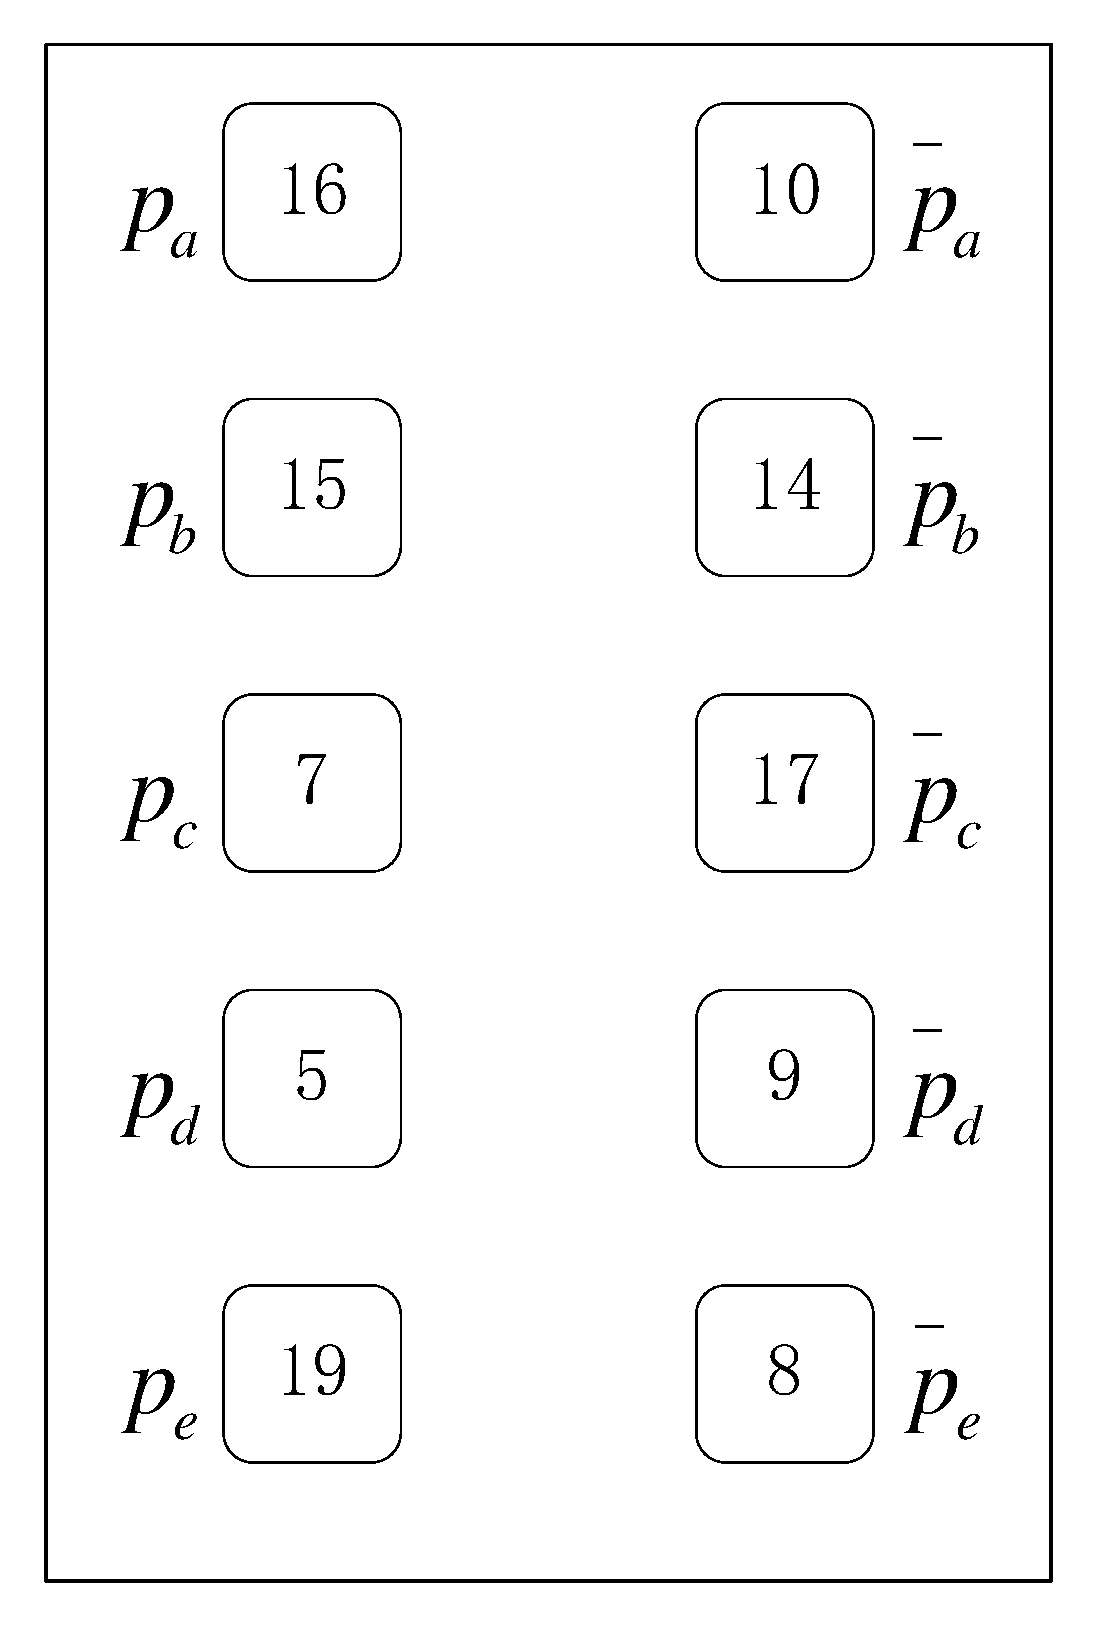
\includegraphics[width=0.32\columnwidth]{fig/partition}
  }
  \subfigure[ $\mathcal{G}_p$上的初始割(作为改进迭代最小割算法的第一步)]
  {
    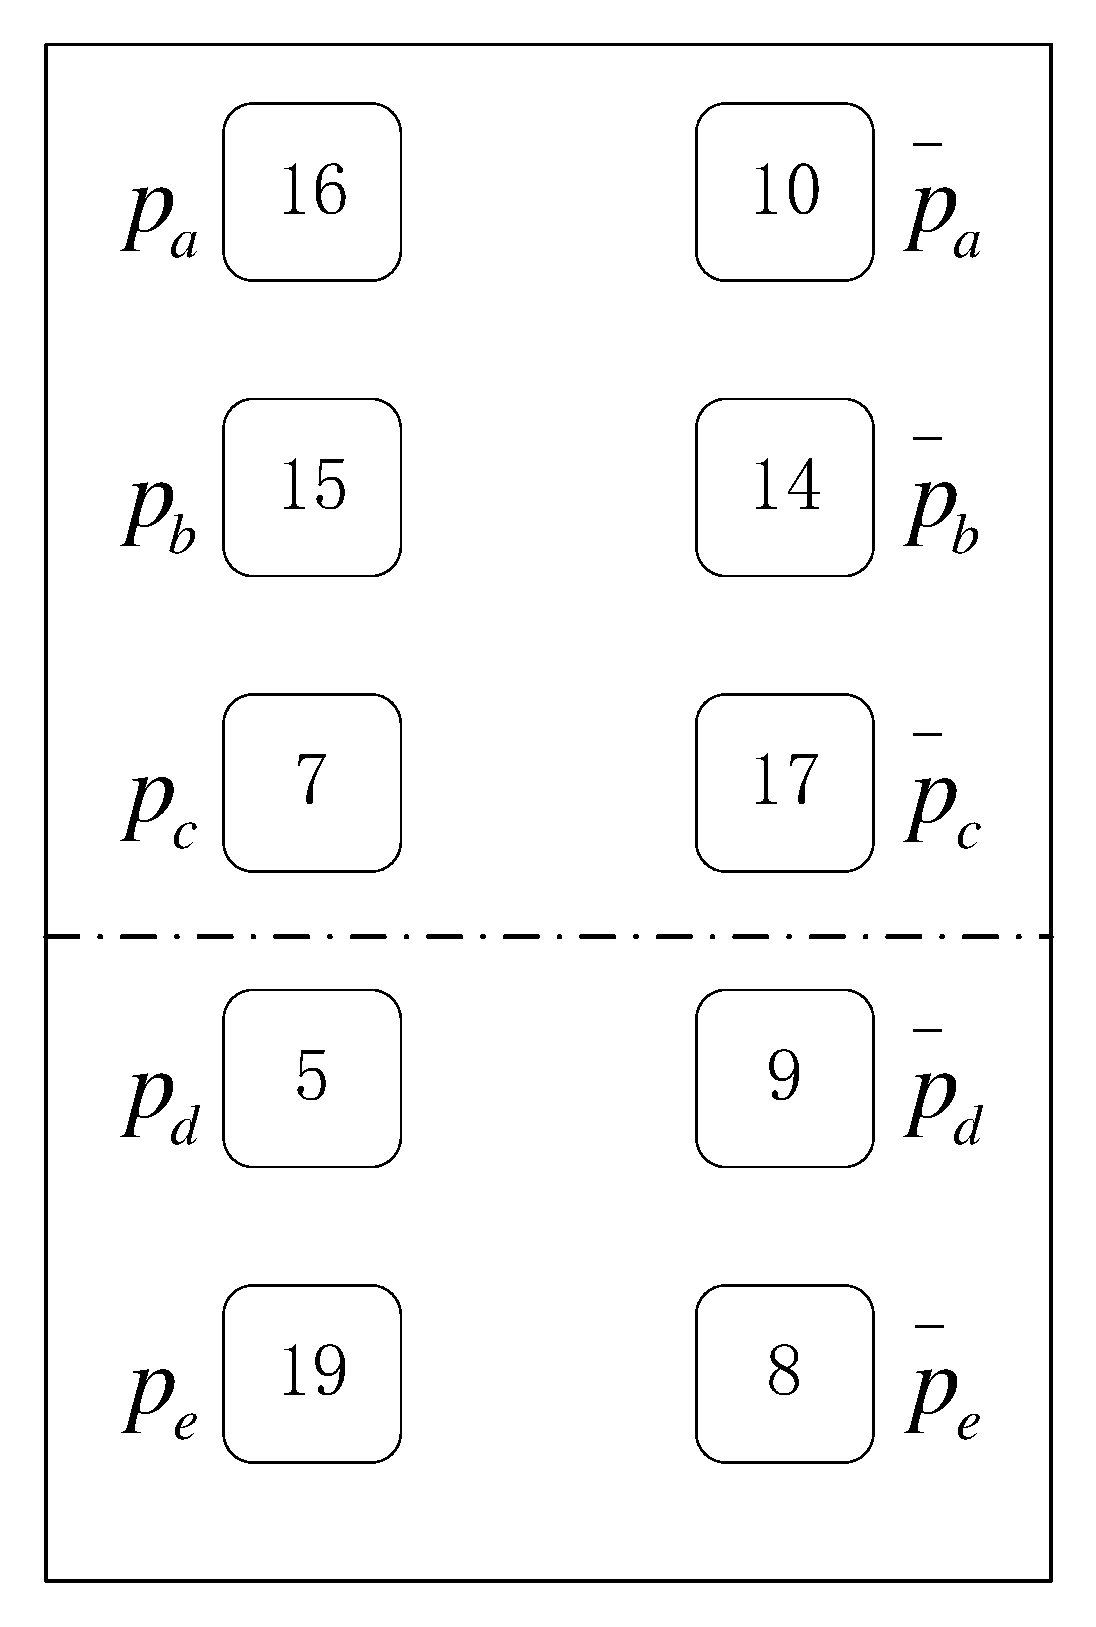
\includegraphics[width=0.32\columnwidth]{fig/partition3}
  }
  \subfigure[$\mathcal{G}_p$上的最小割,然后每个高层块中的二部图匹配]
  {
    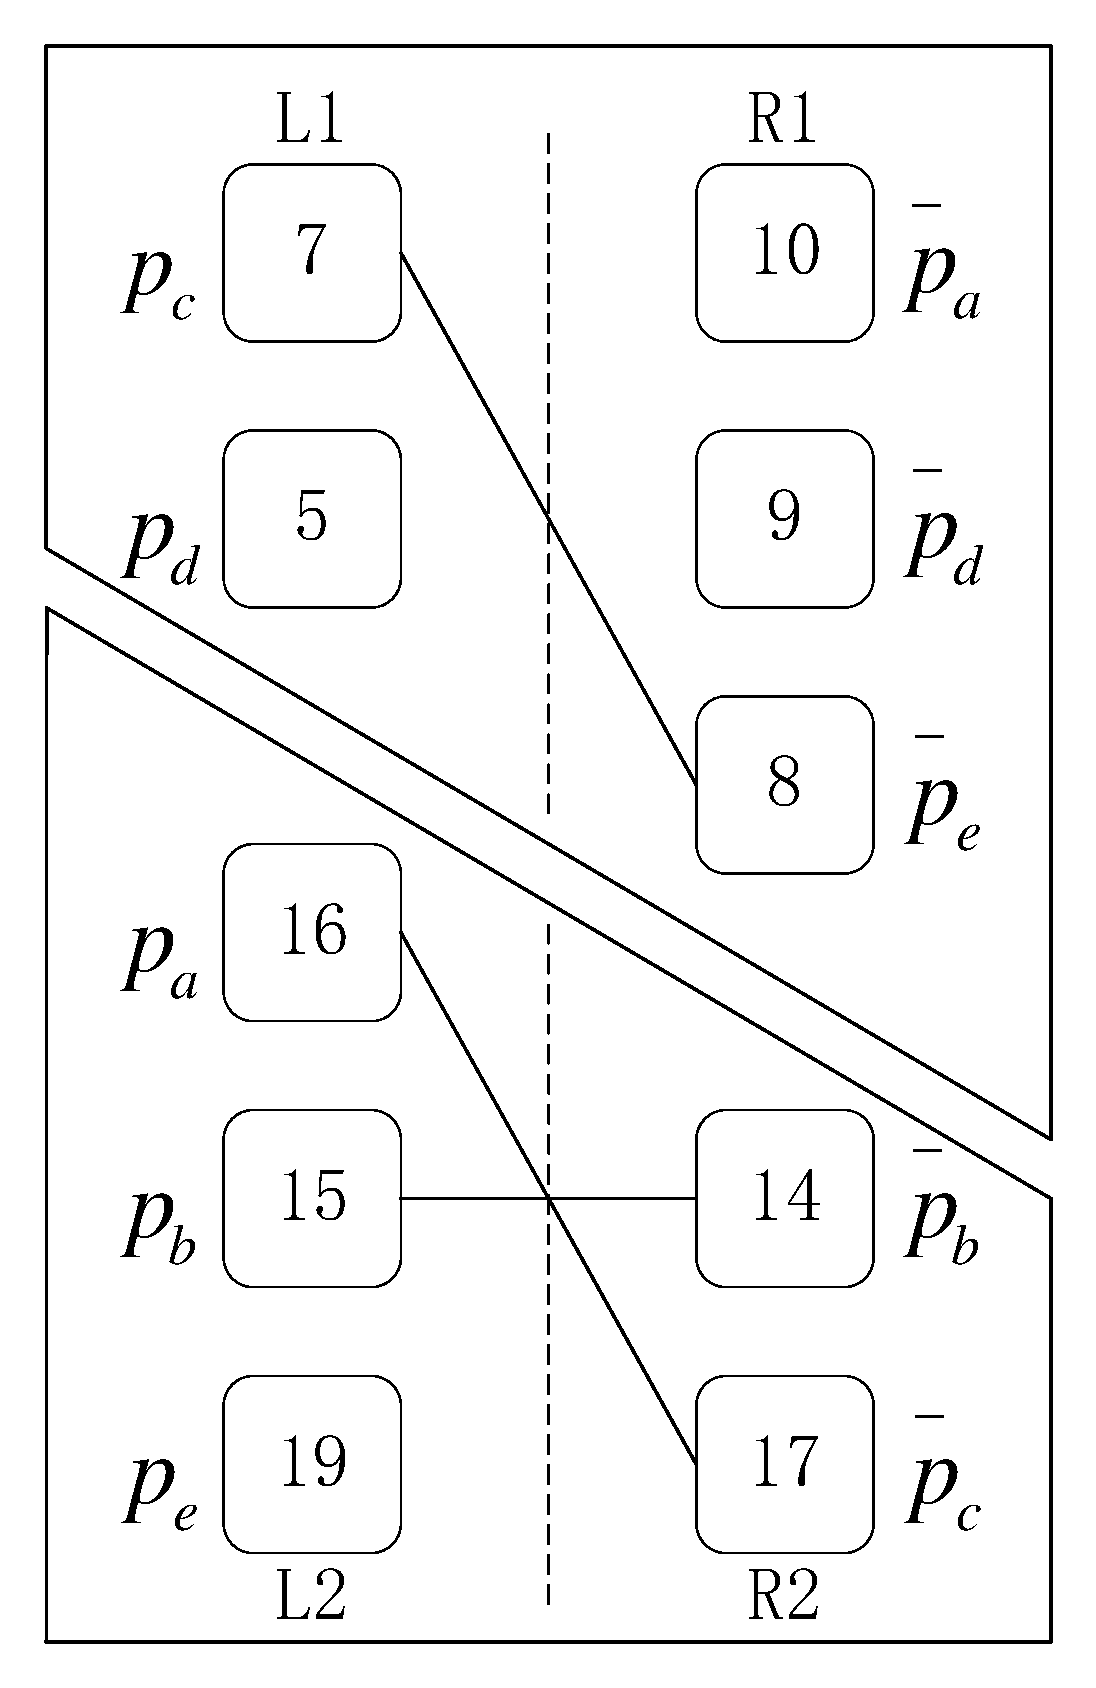
\includegraphics[width=0.32\columnwidth]{fig/match_aft_partition}
  }
  \subfigure[对未匹配的功耗用DVFS做最后调整]
  {
    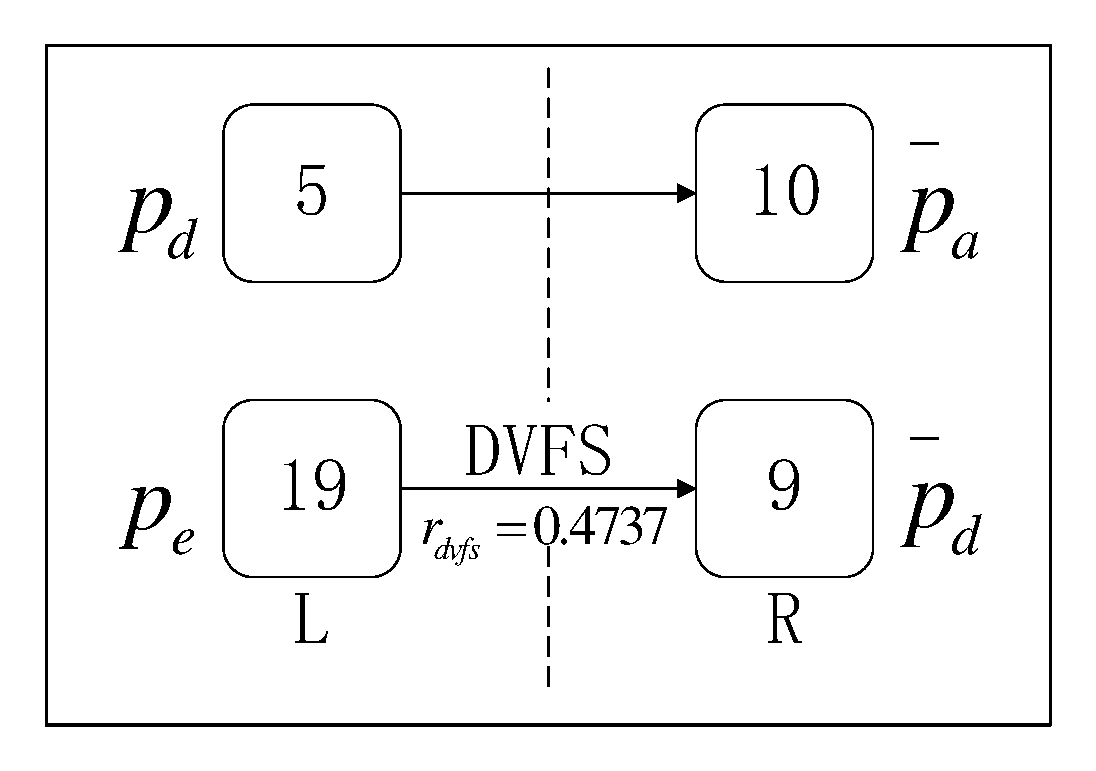
\includegraphics[width=0.32\columnwidth]{fig/DVFS}
  }

  \caption{分层算法在100核微处理器上的高层处理过程示例}\label{fig:partitioning}
\end{figure}

作为一个迭代算法,第一步是做一个初始割,将$V_p$ 分成两个子集 $V_{p1}$ 和 $V_{p2}$。
定义割的权值就是割集的权重的和。图~\ref{fig:partitioning} (b)给出了一个例子,
其中初始割生成了两个子集$V_{p1}=\{P_a, P_b, P_c, \bar{P}_a,
  \bar{P}_b, \bar{P}_c\}$和 $V_{p2}=\{P_d, P_e, \bar{P}_d,
  \bar{P}_e\}$。
  
  然后,为了将正确的元素从一个子集移到另一个子集进行迭代,我们需要测定一个移动操作导致的割的权值变化。
  对每一个元素$v$, 我们首先将元素$v$和相同子集中元素的边集定义为$I(v)$,类似地,将元素$v$和不同子集中的元素的边集定义为$E(v)$。
  将图~\ref{fig:partitioning} (b)中的元素$P_a$做一个例子,
  $I(P_a) = \{(P_a,
    \bar{P}_a), (P_a, \bar{P}_b), (P_a, \bar{P}_c)\}$, $E(P_a) =
  \{(P_a, \bar{P}_d), (P_a, \bar{P}_e, \}$。
  注意这里我们将权重为$0$的边忽略掉,例如 $(P_a, P_b)$等。
  下面是增益函数$f(v)$。
  \begin{equation}
  f(v) = \sum_{n_i \in E(v)}{w(n_i )} - \sum_{n_j \in I(v)}{w(n_j )}.
  \end{equation}
  $f(v)$测定的是如果$v$ 移动到另一个子集,割的权值产生的减少量。
  在这个例子中$f(P_a)$是这样计算的, $f(P_a) =
  (1/|P_a-\bar{P}_d|+1/|P_a-\bar{P}_e|)-(1/|P_a-\bar{P}_a|+1/|P_a-\bar{P}_b|+1/|P_a-\bar{P}_c|)=-1.40$。
  $f(P_a)$是负值表示移动$f(P_a)$到另一个子集的操作会增加割的权值,这就表示$f(P_a)$不应该被移动。
  类似地,其他元素的增益也都被计算了, $f(P_b)=-1.39$, $f(P_c) = 0.92$, $f(P_d) = -0.19$,
  $f(P_e)=0.62$, $f(\bar{P}_a) = -0.39$, $f(\bar{P}_b)=-1.33$,
  $f(\bar{P}_c)=-1.02$, $f(\bar{P}_d) = 0.46$, $f(\bar{P}_e) = 0.84$。
  对第$i$次迭代,最合适的元素记作$v_i$。 $v_i$移动过去之后,将被锁定在那个子集中,不能再移动出来。
  它相邻的元素的增益都要更新。在这个例子中,最合适的元素是$P_c$,$P_c$有最大的增益 $0.92$,
  它将被移动到下面的子集然后锁定。
  在这个简单的例子中,我们可以很容易从图中验证,将$P_c$从上面的子集移动到下面的子集,增强了功耗匹配质量:
$P_c$在下面子集中的$\bar{P}_d$ 和 $\bar{P}_e$有一个更好的匹配候选,比上面子集的任何一个功耗元素都要好。
然而这里有一个问题,在这个例子中如果我们直接执行这个移动操作,每次迭代中都移动最合适的元素可能会导致一个极端不平衡的结果:
一个自己含有很多元素(功耗),另一个子集几乎没有元素。
对我们的方法这个会引起问题,因为如果最小割之后,其中一个块仍然很大,那这个块执行二部图匹配会产生很大的延迟。
所以我们在迭代最小割算法中引入一个平衡阈值:
如果将合适的元素从A移动到B会超出阈值,那它将不被移动。相反的从B中选择最合适的元素移动到A并且锁定。
所有元素都被锁定之后,生成了一个序列,$\mathcal{F} = \{f(v_1), f(v_2), \cdots, f(v_{2m})\}$。
在这个阶段,我们已经移动了所有的元素到对应的另一个子集,这看起来似乎很奇怪,但这不是没有意义的。
实际的情况是,所有的移动操作目的都是为了分析,来确定哪些元素要实际移动,下面步骤继续说明。

在序列 $\mathcal{F}$中,假设所有前面的元素$v_1, v_2, \ldots, v_{i-1}$的移动操作都已经完成, $f(v_i)$表示$v_i$的单步移动操作的增益(割权值的减少)。
所以,为了得出移动$v_1, v_2, \ldots, v_i$的总增益(记作$\tilde{f}(v_i)$),我们需要取和:
\begin{equation}
\tilde{f}(v_i) = \sum\limits_{j=1}^i f(v_j).
\end{equation}
对$i=1,2, \ldots, 2m$分别计算$\tilde{f}(v_i)$,我们形成一个累积和序列,
$\tilde{\mathcal{F}} = \{\tilde{f}(v_1), \tilde{f}(v_2), \cdots,
\tilde{f}(v_{2m})\}$,
其中$\tilde{f}(v_i)$是前面讨论过的元素$v_1$ 到 $v_i$移动的总增益。
假设 $\tilde{f}(v_k)$是$\tilde{F}$中的最大元素,这意味着移动$v_1, v_2, \ldots, v_k$可以得到最大的增益(即最大减小割权值)。
这样,我们就执行实际的操作,移动$\{v_1, v_2, \cdots, v_k\}$去它对应的另一个子集。
所有上面的程序记为一个移动动作。

尽管移动动作可以重复执行,但是以前在电路分割上的研究已经表明2到4次的移动动作已经足够实现最小化。对我们这个情况,实验表明执行一次移动动作已经足够了。

最小割之后,我们将所有剩余功耗分割成块。然后二部图匹配可以在每块内部执行。
因为最小割已经将相关的功耗划到了同一块中,执行二部图匹配之后剩下的未匹配的功耗在其他块中也很难找到匹配了。
所以,不在执行更进一步的二部图匹配了,我们可以由之前的低层和高层的二部图匹配结果直接确定任务迁移操作。
最后没有匹配上的功耗,可以简单的用DVFS进行处理。

图~\ref{fig:partitioning} (a), (b) 和(c)展示了高层的匹配的一个例子。
在图~\ref{fig:partitioning} (a)中,低层匹配(图~\ref{fig:cpu_partition} (b)表示已表示出)之后未匹配上的功耗全部收集形成图 $\mathcal{G}_p$。
注意,图 $\mathcal{G}_p$ 中所有的元素都有带权重的边连接,图~\ref{fig:partitioning}中为简化并没有表示出。
图 $\mathcal{G}_p$的初始割由图~\ref{fig:partitioning} (b)上的虚线表示。然后执行迭代最小割算法,
图~\ref{fig:partitioning} (c)表示$\mathcal{G}_p$的最终割,$\mathcal{G}_p$中的功耗元素被分割成了两个块,
然后,每个新块的形成一个二部图,高层二部图匹配在每个新块执行。


\section{DVFS最终调整}\label{sec:dvfs_adj}



















































